%% AMS-LaTeX Created with the Wolfram Language : www.wolfram.com

%\documentclass{article}
%\usepackage{amsmath, amssymb, graphics, setspace}

%\newcommand{\mathsym}[1]{{}}
%\newcommand{\unicode}[1]{{}}
\chapter{Mathematica File: Kronig-Penney Model}{\label{Mathematica File: Kronig-Penney Model}

\newcounter{mathematicapage}

\begin{doublespace}
\noindent\(\pmb{\text{(*} \text{Kronig}-\text{Penney} \text{model} \text{using} \text{transfer} \text{matrix} \text{as} \text{in} \text{notes} \text{by}
\text{Geshjkenbein}, p.6 \text{ff} \text{*)}}\)
\end{doublespace}

\begin{doublespace}
\noindent\(\pmb{\text{Clear}[\text{ell},q,p,\text{epsilon},m]\text{     }}\)
\end{doublespace}

\begin{doublespace}
\noindent\(\pmb{\text{ell}\text{:=}\{\{1,1\},\{I q, -I q\}\}\text{      }\text{(* matrix L *)}}\)
\end{doublespace}

\begin{doublespace}
\noindent\(\pmb{\text{MatrixForm}[\text{ell}]}\)
\end{doublespace}

\begin{doublespace}
\noindent\(\left(
\begin{array}{cc}
 1 & 1 \\
 i q & -i q \\
\end{array}
\right)\)
\end{doublespace}

\begin{doublespace}
\noindent\(\pmb{v\text{:=}\{\{1,0\},\{\text{epsilon}, 1\}\}\text{    }\text{(*} \text{matrix} V, \text{epsilon} \text{as} \text{defined} \text{in}
\text{Section} 2.2 \text{*)}}\)
\end{doublespace}

\begin{doublespace}
\noindent\(\pmb{\text{MatrixForm}[v]}\)
\end{doublespace}

\begin{doublespace}
\noindent\(\left(
\begin{array}{cc}
 1 & 0 \\
 \text{epsilon} & 1 \\
\end{array}
\right)\)
\end{doublespace}

\begin{doublespace}
\noindent\(\pmb{p\text{:=}\{\{\text{Exp}[I q],0\},\{0,\text{Exp}[-I q]\}\}\text{    }\text{(*} \text{matrix} P, \text{called} T \text{in} \text{Geshjkenbein}\text{
 }\text{*)} }\)
\end{doublespace}

\begin{doublespace}
\noindent\(\pmb{\text{MatrixForm}[p]}\)
\end{doublespace}

\begin{doublespace}
\noindent\(\left(
\begin{array}{cc}
 e^{i q} & 0 \\
 0 & e^{-i q} \\
\end{array}
\right)\)
\end{doublespace}

\begin{doublespace}
\noindent\(\pmb{t\text{:=}p.\text{Inverse}[\text{ell},\text{Method}\text{-$>$}\text{{``}CofactorExpansion{''}}].v.\text{ell}\text{   }\text{(* transfer
matrix T *)}}\)
\end{doublespace}

\begin{doublespace}
\noindent\(\pmb{\text{MatrixForm}[t]}\)
\end{doublespace}

\begin{doublespace}
\noindent\(\left(
\begin{array}{cc}
 e^{i q}-\frac{i e^{i q} \text{epsilon}}{2 q} & -\frac{i e^{i q} \text{epsilon}}{2 q} \\
 \frac{i e^{-i q} \text{epsilon}}{2 q} & e^{-i q}+\frac{i e^{-i q} \text{epsilon}}{2 q} \\
\end{array}
\right)\)
\end{doublespace}

\begin{doublespace}
\noindent\(\pmb{\text{Det}[t]}\)
\end{doublespace}

\begin{doublespace}
\noindent\(1\)
\end{doublespace}

\begin{doublespace}
\noindent\(\pmb{\text{}}\)
\end{doublespace}

\begin{doublespace}
\noindent\(\pmb{\text{(* Eigenvectors of transfer matrix t *)}}\)
\end{doublespace}

\begin{doublespace}
\noindent\(\pmb{\text{Eigenvectors}[t]}\)
\end{doublespace}

\begin{doublespace}
\noindent\(\left\{\left\{-\frac{\text{epsilon}+e^{2 i q} \text{epsilon}-2 i q+2 i e^{2 i q} q-i \sqrt{-16 e^{2 i q} q^2+\left(-i \text{epsilon}+i
e^{2 i q} \text{epsilon}-2 q-2 e^{2 i q} q\right)^2}}{2 \text{epsilon}},1\right\},
\newline
\left\{-\frac{\text{epsilon}+e^{2 i q} \text{epsilon}-2 i q+2 i
e^{2 i q} q+i \sqrt{-16 e^{2 i q} q^2+\left(-i \text{epsilon}+i e^{2 i q} \text{epsilon}-2 q-2 e^{2 i q} q\right)^2}}{2 \text{epsilon}},1\right\}\right\}\)
\end{doublespace}

\begin{doublespace}
\noindent\(\pmb{\text{(* pasted from above *)}}\)
\end{doublespace}

\begin{doublespace}
\noindent\(\pmb{\text{va1}[\text{q$\_$},\text{epsilon$\_$}]\text{:=}\left\{-\frac{\text{epsilon}+e^{2 i q} \text{epsilon}-2 i q+2 i e^{2 i q} q-i
\sqrt{-16 e^{2 i q} q^2+\left(-i \text{epsilon}+i e^{2 i q} \text{epsilon}-2 q-2 e^{2 i q} q\right)^2}}{2 \text{epsilon}},1\right\}}\)
\end{doublespace}

\begin{doublespace}
\noindent\(\pmb{\text{v1}[\text{q$\_$},\text{epsilon$\_$}]\text{:=}\text{va1}[q,\text{epsilon}]/\text{Norm}[\text{va1}[q,\text{epsilon}]]\text{ 
   }\text{(*} \text{normalized} \text{*)}}\)
\end{doublespace}

\begin{doublespace}
\noindent\(\pmb{\text{va2}[\text{q$\_$},\text{epsilon$\_$}]\text{:=}\left\{-\frac{\text{epsilon}+e^{2 i q} \text{epsilon}-2 i q+2 i e^{2 i q} q+i
\sqrt{-16 e^{2 i q} q^2+\left(-i \text{epsilon}+i e^{2 i q} \text{epsilon}-2 q-2 e^{2 i q} q\right)^2}}{2 \text{epsilon}},1\right\}}\)
\end{doublespace}

\begin{doublespace}
\noindent\(\pmb{\text{v2}[\text{q$\_$},\text{epsilon$\_$}]\text{:=}\text{va2}[q,\text{epsilon}]/\text{Norm}[\text{va2}[q,\text{epsilon}]]\text{ 
}}\)
\end{doublespace}

\begin{doublespace}
\noindent\(\pmb{\text{}}\)
\end{doublespace}

\begin{doublespace}
\noindent\(\pmb{\text{(* Simplified form of above eigenvectors *)}}\)
\end{doublespace}

\begin{doublespace}
\noindent\(\pmb{\text{qq}[\text{q$\_$},\text{epsilon$\_$}]\text{:=}\text{Cos}[q]+(\text{epsilon}/(2q))\text{Sin}[q] }\)
\end{doublespace}

\begin{doublespace}
\noindent\(\pmb{\text{ww}[\text{q$\_$},\text{epsilon$\_$}]\text{:=}-\text{Cos}[q]+(2q/\text{epsilon}) \text{Sin}[q]}\)
\end{doublespace}

\begin{doublespace}
\noindent\(\pmb{\text{vv1}[\text{q$\_$},\text{epsilon$\_$}]\text{:=} \{\text{Exp}[I q](\text{ww}[q,\text{epsilon}]+(2q/\text{epsilon})\text{Sqrt}[1-\text{qq}[q,\text{epsilon}]{}^{\wedge}2]),1\}}\)
\end{doublespace}

\begin{doublespace}
\noindent\(\pmb{\text{vv2}[\text{q$\_$},\text{epsilon$\_$}]\text{:=} \{\text{Exp}[I q](\text{ww}[q,\text{epsilon}]-(2q/\text{epsilon})\text{Sqrt}[1-\text{qq}[q,\text{epsilon}]{}^{\wedge}2]),1\}}\)
\end{doublespace}

\begin{doublespace}
\noindent\(\pmb{\text{}}\)
\end{doublespace}

\begin{doublespace}
\noindent\(\pmb{\text{(*} \text{Check} \text{that} \text{vv1} = \text{va1}, \text{vv2} = \text{va2} \text{*)}}\)
\end{doublespace}

\begin{doublespace}
\noindent\(\pmb{\text{va1}[0.7,0.1]}\)
\end{doublespace}

\begin{doublespace}
\noindent\(\{12.5798\, +10.5958 i,1\}\)
\end{doublespace}

\begin{doublespace}
\noindent\(\pmb{\text{vv1}[0.7,0.1]}\)
\end{doublespace}

\begin{doublespace}
\noindent\(\{12.5798\, +10.5958 i,1\}\)
\end{doublespace}

\begin{doublespace}
\noindent\(\pmb{\text{va2}[0.7,0.1]}\)
\end{doublespace}

\begin{doublespace}
\noindent\(\{0.0465017\, +0.0391679 i,1\}\)
\end{doublespace}

\begin{doublespace}
\noindent\(\pmb{\text{vv2}[0.7,0.1]}\)
\end{doublespace}

\begin{doublespace}
\noindent\(\{0.0465017\, +0.0391679 i,1\}\)
\end{doublespace}

\begin{doublespace}
\noindent\(\pmb{\text{(* End check *)}}\)
\end{doublespace}

\begin{doublespace}
\noindent\(\pmb{\text{}}\)
\end{doublespace}

\begin{doublespace}
\noindent\(\pmb{\text{(*} \text{Modified}, \text{normalized} \text{eigenvectors} \text{to} \text{be} \text{used} \text{in} \text{the} \text{following}
\text{*)}}\)
\end{doublespace}

\begin{doublespace}
\noindent\(\pmb{\text{v1norm}[\text{q$\_$},\text{epsilon$\_$}]\text{:=}\text{vv1}[q,\text{epsilon}]/\text{Norm}[\text{vv1}[q,\text{epsilon}]]}\)
\end{doublespace}

\begin{doublespace}
\noindent\(\pmb{\text{v2norm}[\text{q$\_$},\text{epsilon$\_$}]\text{:=}\text{Exp}[-I q]\text{  }\text{vv2}[q,\text{epsilon}]/\text{Norm}[\text{vv2}[q,\text{epsilon}]]\text{
   }\text{(*} \text{note} \text{factor} \text{Exp}[-I q] \text{*)}}\)
\end{doublespace}

\begin{doublespace}
\noindent\(\pmb{\text{(*} \text{v1norm}[[1]]+\text{v1norm}[[2]] \text{and} \text{v2norm}[[1]]+\text{v2norm}[[2]] \text{are} \text{complex} \text{conjugate},
}\\
\pmb{\text{   }\text{but} \text{only} \text{with} \text{factor} \text{Exp}[-I q] \text{in} \text{v2norm} \text{included}. \text{This} \text{is} \text{the}
\text{modification}. \text{*)}}\)
\end{doublespace}

\begin{doublespace}
\noindent\(\pmb{\text{v1norm}[0.7,0.1][[1]]+\text{v1norm}[0.7,0.1][[2]]}\)
\end{doublespace}

\begin{doublespace}
\noindent\(0.82412\, +0.64303 i\)
\end{doublespace}

\begin{doublespace}
\noindent\(\pmb{\text{v2norm}[0.7,0.1][[1]]+\text{v2norm}[0.7,0.1][[2]]}\)
\end{doublespace}

\begin{doublespace}
\noindent\(0.82412\, -0.64303 i\)
\end{doublespace}

\begin{doublespace}
\noindent\(\pmb{\text{(*} \text{alternative} \text{form} \text{of} \text{v2norm}, \text{further} \text{simplified} \text{*)}}\)
\end{doublespace}

\begin{doublespace}
\noindent\(\pmb{\text{vv2alt}[\text{q$\_$},\text{epsilon$\_$}]\text{:=} \{\text{ww}[q,\text{epsilon}]-(2q/\text{epsilon})\text{Sqrt}[1-\text{qq}[q,\text{epsilon}]{}^{\wedge}2],\text{Exp}[-I
q]\}}\)
\end{doublespace}

\begin{doublespace}
\noindent\(\pmb{\text{v2normalt}[\text{q$\_$}, \text{epsilon$\_$}]\text{:=}\text{vv2alt}[q,\text{epsilon}]/\text{Norm}[\text{vv2alt}[q,\text{epsilon}]]}\)
\end{doublespace}

\begin{doublespace}
\noindent\(\pmb{\text{v2normalt}[0.7, 0.1][[1]]+\text{v2normalt}[0.7, 0.1][[2]]}\)
\end{doublespace}

\begin{doublespace}
\noindent\(0.82412\, -0.64303 i\)
\end{doublespace}

\begin{doublespace}
\noindent\(\pmb{\text{}}\)
\end{doublespace}

\begin{doublespace}
\noindent\(\pmb{\text{(*} \text{Eigenvalues} \text{mu} \text{of} \text{transfer} \text{matrix} t, \text{cp}. \text{Geshkenbein}, \text{Eq}. (50)
\text{*)}}\)
\end{doublespace}

\begin{doublespace}
\noindent\(\pmb{\text{Eigenvalues}[t]}\)
\end{doublespace}

\begin{doublespace}
\noindent\(\left\{\frac{e^{-i q} \left(i \text{epsilon}-i e^{2 i q} \text{epsilon}+2 q+2 e^{2 i q} q-\sqrt{-16 e^{2 i q} q^2+\left(-i \text{epsilon}+i
e^{2 i q} \text{epsilon}-2 q-2 e^{2 i q} q\right)^2}\right)}{4 q},\frac{e^{-i q} \left(i \text{epsilon}-i e^{2 i q} \text{epsilon}+2 q+2 e^{2 i q}
q+\sqrt{-16 e^{2 i q} q^2+\left(-i \text{epsilon}+i e^{2 i q} \text{epsilon}-2 q-2 e^{2 i q} q\right)^2}\right)}{4 q}\right\}\)
\end{doublespace}

\begin{doublespace}
\noindent\(\pmb{\text{(*} => \text{mu} = \exp (+/- i k), \cos (k) = \cos (q) + \text{epsilon}/(2q) \sin (q) =: Q(q) \text{*)}}\)
\end{doublespace}

\begin{doublespace}
\noindent\(\pmb{\text{Plot}[\text{ArcCos}[x],\{x,-1,1\}]}\)
\end{doublespace}

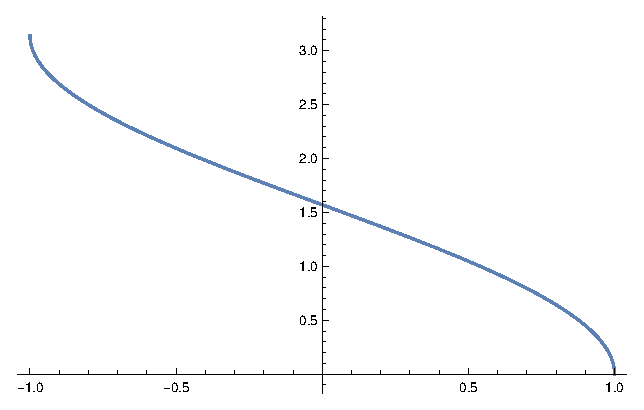
\includegraphics{chapters/appendices/KP_Mathematica/Kronig_Penney_model_transfer_matrix_gr1.eps}

\begin{doublespace}
\noindent\(\pmb{\text{kk}[\text{q$\_$},\text{epsilon$\_$}]\text{:=}\text{ArcCos}[\text{qq}[q,\text{epsilon}]]\text{                             }\text{(*
0 $<$ k $<$ Pi *)} }\)
\end{doublespace}

\begin{doublespace}
\noindent\(\pmb{\text{}}\\
\pmb{}\)
\end{doublespace}

\begin{doublespace}
\noindent\(\pmb{\text{(*} \text{Illustration}: \text{plot} \text{band} \text{structure} q(k) = \text{omega}(k)/v \text{for} -\text{Pi}<k<\text{Pi}
\text{in} \text{reduced} \text{zone} \text{scheme} \text{*)}}\\
\pmb{\text{(*} \text{for} \text{epsilon} = 1 \text{*)}}\)
\end{doublespace}

\begin{doublespace}
\noindent\(\pmb{\text{Plot}[\text{kk}[q,1],\{q,0,14\}]\text{         }\text{(*} \text{function} k(q), \text{range} 0 < k < \text{Pi}, \text{epsilon}
= 1 \text{*)} }\)
\end{doublespace}

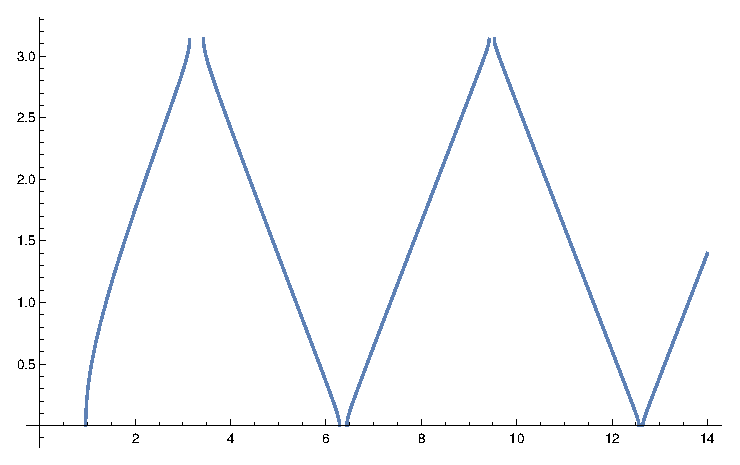
\includegraphics{chapters/appendices/KP_Mathematica/Kronig_Penney_model_transfer_matrix_gr2.eps}

\begin{doublespace}
\noindent\(\pmb{\text{kq}[\text{q$\_$},\text{epsilon$\_$}]\text{:=}\text{If}[\text{Abs}[\text{qq}[q,\text{epsilon}]]<1,\text{kk}[q,\text{epsilon}],100]\text{
    }\text{(*} k(q), \text{allow} \text{only} |q|<1 \text{*)}}\)
\end{doublespace}

\begin{doublespace}
\noindent\(\pmb{\text{(*} \text{use} \text{parametric} \text{plot} \text{to} \text{plot} \text{inverse} \text{function} q(k) \text{*)}}\)
\end{doublespace}

\begin{doublespace}
\noindent\(\pmb{\text{pos}=\text{ParametricPlot}[\{\text{kq}[q,1],q\},\{q,0,14\},\text{PlotRange}\to \{\{-\text{Pi}-0.1,\text{Pi}+0.1\},\{0,14\}\},}\\
\pmb{\text{PlotStyle}\to \{\{\text{Black},\text{Thickness}[0.007]\}\}, \text{AxesStyle}\to \text{Directive}[20],\text{Ticks}\to \{\{-\text{Pi},0,\text{Pi}\},\{2,4,8,10\}\}]}\)
\end{doublespace}

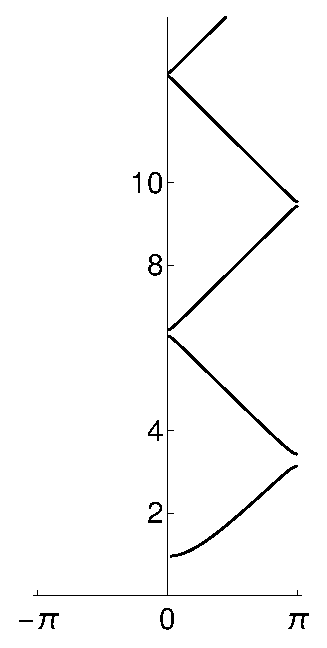
\includegraphics{chapters/appendices/KP_Mathematica/Kronig_Penney_model_transfer_matrix_gr3.eps}
\begin{doublespace}
\noindent\(\pmb{\text{neg}=\text{ParametricPlot}[\{-\text{kq}[q,1],q\},\{q,0,14\},\text{PlotRange}\to \{\{-\text{Pi}-0.1,\text{Pi}+0.1\},\{0,14\}\},}\\
\pmb{\text{PlotStyle}\to \{\{\text{Black},\text{Thickness}[0.007]\}\}, \text{AxesStyle}\to \text{Directive}[20],\text{Ticks}\to \{\{-\text{Pi},0,\text{Pi}\},\{2,4,8,10\}\}]}\)
\end{doublespace}

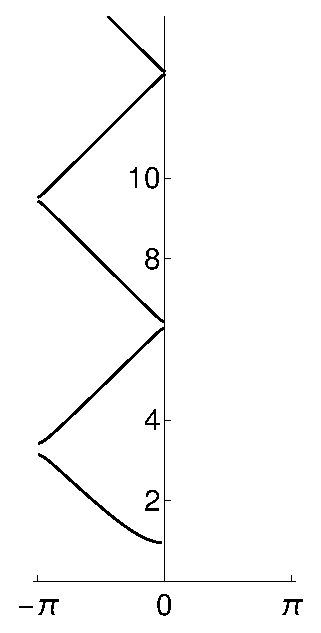
\includegraphics{chapters/appendices/KP_Mathematica/Kronig_Penney_model_transfer_matrix_gr4.eps}

\begin{doublespace}
\noindent\(\pmb{\text{pipos}=\text{ParametricPlot}[\{\text{Pi},q\},\{q,0,14\},\text{PlotRange}\to \{\{-\text{Pi}-0.1,\text{Pi}+0.1\},\{0,14\}\},\text{PlotStyle}\to
\{\{\text{Black},\text{Thickness}[0.0015]\}\}, }\\
\pmb{\text{AxesStyle}\to \text{Directive}[20],\text{Ticks}\to \{\{-\text{Pi},0,\text{Pi}\},\{2,4,8,10\}\}]}\)
\end{doublespace}

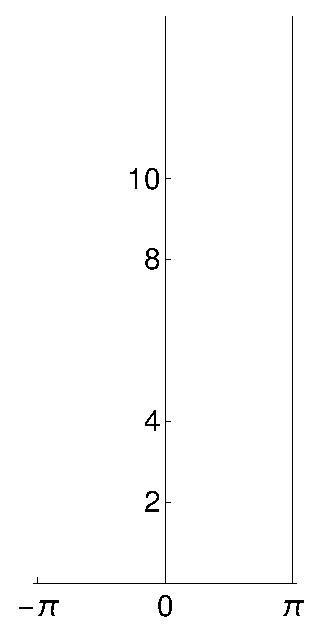
\includegraphics{chapters/appendices/KP_Mathematica/Kronig_Penney_model_transfer_matrix_gr5.eps}

\begin{doublespace}
\noindent\(\pmb{\text{pineg}=\text{ParametricPlot}[\{-\text{Pi},q\},\{q,0,14\},\text{PlotRange}\to \{\{-\text{Pi}-0.1,\text{Pi}+0.1\},\{0,14\}\},\text{PlotStyle}\to
\{\{\text{Black},\text{Thickness}[0.0015]\}\}, }\\
\pmb{\text{AxesStyle}\to \text{Directive}[20],\text{Ticks}\to \{\{-\text{Pi},0,\text{Pi}\},\{2,4,8,10\}\}]}\)
\end{doublespace}

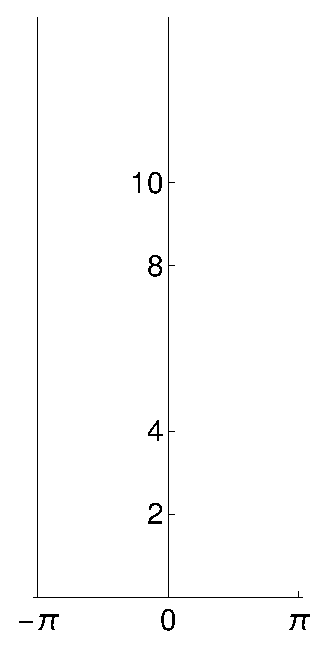
\includegraphics{chapters/appendices/KP_Mathematica/Kronig_Penney_model_transfer_matrix_gr6.eps}

\begin{doublespace}
\noindent\(\pmb{\text{band}=\text{Show}[\text{neg},\text{pos},\text{pipos},\text{pineg}]}\)
\end{doublespace}

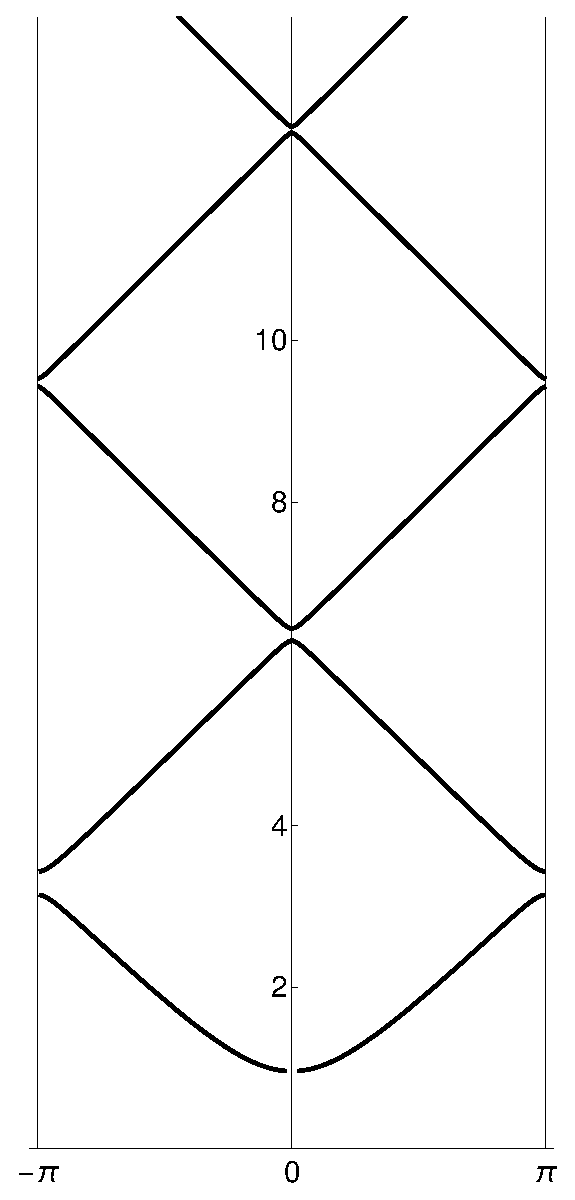
\includegraphics{chapters/appendices/KP_Mathematica/Kronig_Penney_model_transfer_matrix_gr7.eps}

\begin{doublespace}
\noindent\(\pmb{\text{Export}[\text{{``}bs.png{''}},\text{band},\text{ImageResolution}\to 300]}\)
\end{doublespace}

\begin{doublespace}
\noindent\(\text{bs.png}\)
\end{doublespace}

\begin{doublespace}
\noindent\(\pmb{\text{(* End Illustration *)}}\)
\end{doublespace}

\begin{doublespace}
\noindent\(\pmb{\text{}}\)
\end{doublespace}

\begin{doublespace}
\noindent\(\pmb{\text{(*} \text{Bloch} \text{functions} \text{Phi}(x) \text{with} \text{additional} \text{normalization} \text{*)} }\)
\end{doublespace}

\begin{doublespace}
\noindent\(\pmb{\text{(*} \text{allow} \text{only} |q|<1 \text{*)}}\)
\end{doublespace}

\begin{doublespace}
\noindent\(\pmb{\text{(*} \text{in} \text{what} \text{follows}: \text{index} 1 = +k, \text{index} 2 = -k \text{*)}}\)
\end{doublespace}

\begin{doublespace}
\noindent\(\pmb{\text{exp1}[\text{q$\_$},\text{epsilon$\_$},\text{n$\_$}]\text{:=}\text{If}[\text{Abs}[\text{qq}[q,\text{epsilon}]]<1,\text{Exp}[I
\text{kk}[q,\text{epsilon}] n],0]\text{      }\text{(* k1 $>$ 0 *)}}\)
\end{doublespace}

\begin{doublespace}
\noindent\(\pmb{\text{exp2}[\text{q$\_$},\text{epsilon$\_$},\text{n$\_$}]\text{:=}\text{If}[\text{Abs}[\text{qq}[q,\text{epsilon}]]<1,\text{Exp}[-I
\text{kk}[q,\text{epsilon}] n],0]\text{   }\text{(*} \text{k2} = -\text{k1} < 0 \text{*)}}\)
\end{doublespace}

\begin{doublespace}
\noindent\(\pmb{\text{(*} \text{phi1raw}, \text{phi2raw} \text{not} \text{correctly} \text{normalized}, \text{missing} \text{normalization} \text{factors}
\text{norm1}, \text{norm2} \text{below} \text{*)}}\)
\end{doublespace}

\begin{doublespace}
\noindent\(\pmb{\text{phi1raw}[\text{x$\_$},\text{n$\_$},\text{q$\_$},\text{epsilon$\_$}]\text{:=}}\\
\pmb{\text{exp1}[q,\text{epsilon},n] (\text{v1norm}[q,\text{epsilon}][[1]]\text{Exp}[I q (x-n)]+\text{v1norm}[q,\text{epsilon}][[2]]\text{Exp}[-I
q (x-n)])/}\\
\pmb{(\text{v1norm}[q,\text{epsilon}][[1]]+\text{v1norm}[q,\text{epsilon}][[2]])}\)
\end{doublespace}

\begin{doublespace}
\noindent\(\pmb{\text{phi2raw}[\text{x$\_$},\text{n$\_$},\text{q$\_$},\text{epsilon$\_$}]\text{:=}}\\
\pmb{\text{exp2}[q,\text{epsilon},n] (\text{v2norm}[q,\text{epsilon}][[1]]\text{Exp}[I q (x-n)]+\text{v2norm}[q,\text{epsilon}][[2]]\text{Exp}[-I
q (x-n)])/}\\
\pmb{(\text{v2norm}[q,\text{epsilon}][[1]]+\text{v2norm}[q,\text{epsilon}][[2]])}\)
\end{doublespace}

\begin{doublespace}
\noindent\(\pmb{\text{}}\)
\end{doublespace}

\begin{doublespace}
\noindent\(\pmb{\text{}}\)
\end{doublespace}

\begin{doublespace}
\noindent\(\pmb{\text{(*} \text{functions} u(x) \text{for} 0<x<1, \text{then} \text{periodically} \text{extended} \text{*)}}\)
\end{doublespace}

\begin{doublespace}
\noindent\(\pmb{\text{u1raw}[\text{x$\_$},\text{q$\_$},\text{epsilon$\_$}]\text{:=}}\\
\pmb{(\text{v1norm}[q,\text{epsilon}][[1]]\text{Exp}[I (q-\text{kk}[q,\text{epsilon}])(x-1)]+\text{v1norm}[q,\text{epsilon}][[2]]\text{Exp}[-I (q+\text{kk}[q,\text{epsilon}])(x-1)])/}\\
\pmb{(\text{v1norm}[q,\text{epsilon}][[1]]+\text{v1norm}[q,\text{epsilon}][[2]])}\)
\end{doublespace}

\begin{doublespace}
\noindent\(\pmb{\text{norm1}[\text{q$\_$},\text{epsilon$\_$}] \text{:=}\text{Sqrt}[\text{NIntegrate}[\text{u1raw}[x,q,\text{epsilon}]\text{Conjugate}[\text{u1raw}[x,q,\text{epsilon}]],\{x,0,1\}]]}\)
\end{doublespace}

\begin{doublespace}
\noindent\(\pmb{\text{u1}[\text{x$\_$},\text{q$\_$},\text{epsilon$\_$}] \text{:=}\text{u1raw}[x,q,\text{epsilon}]/\text{norm1}[q,\text{epsilon}]\text{
     }}\)
\end{doublespace}

\begin{doublespace}
\noindent\(\pmb{\text{NIntegrate}[\text{u1}[x,0.3,0.7]\text{Conjugate}[\text{u1}[x,0.3,0.7]],\{x,0,1\}]\text{      }\text{(* u1 correctly normalized
*)} }\)
\end{doublespace}

\begin{doublespace}
\noindent\(1.\)
\end{doublespace}

\begin{doublespace}
\noindent\(\pmb{\text{u2raw}[\text{x$\_$},\text{q$\_$},\text{epsilon$\_$}]\text{:=}}\\
\pmb{(\text{v2norm}[q,\text{epsilon}][[1]]\text{Exp}[I (q+\text{kk}[q,\text{epsilon}])(x-1)]+\text{v2norm}[q,\text{epsilon}][[2]]\text{Exp}[-I (q-\text{kk}[q,\text{epsilon}])(x-1)])/}\\
\pmb{(\text{v2norm}[q,\text{epsilon}][[1]]+\text{v2norm}[q,\text{epsilon}][[2]])}\)
\end{doublespace}

\begin{doublespace}
\noindent\(\pmb{\text{norm2}[\text{q$\_$},\text{epsilon$\_$}] \text{:=}\text{Sqrt}[\text{NIntegrate}[\text{u2raw}[x,q,\text{epsilon}]\text{Conjugate}[\text{u2raw}[x,q,\text{epsilon}]],\{x,0,1\}]]}\)
\end{doublespace}

\begin{doublespace}
\noindent\(\pmb{\text{u2}[\text{x$\_$},\text{q$\_$},\text{epsilon$\_$}] \text{:=}\text{u2raw}[x,q,\text{epsilon}]/\text{norm2}[q,\text{epsilon}]}\)
\end{doublespace}

\begin{doublespace}
\noindent\(\pmb{\text{NIntegrate}[\text{u2}[x,0.3,0.7]\text{Conjugate}[\text{u2}[x,0.3,0.7]],\{x,0,1\}]\text{      }\text{(* u2 correctly normalized
*)} }\)
\end{doublespace}

\begin{doublespace}
\noindent\(1.\)
\end{doublespace}

\begin{doublespace}
\noindent\(\pmb{\text{}}\)
\end{doublespace}

\begin{doublespace}
\noindent\(\pmb{\text{(*} \text{functions} c(q), d(q) \text{*)} }\)
\end{doublespace}

\begin{doublespace}
\noindent\(\pmb{\text{u1prime}[\text{x$\_$},\text{q$\_$},\text{epsilon$\_$}]\text{:=}\text{Derivative}[1,0,0][\text{u1raw}][x,q,\text{epsilon}]/\text{norm1}[q,\text{epsilon}]}\)
\end{doublespace}

\begin{doublespace}
\noindent\(\pmb{\text{u2prime}[\text{x$\_$},\text{q$\_$},\text{epsilon$\_$}]\text{:=}\text{Derivative}[1,0,0][\text{u2raw}][x,q,\text{epsilon}]/\text{norm2}[q,\text{epsilon}]}\)
\end{doublespace}

\begin{doublespace}
\noindent\(\pmb{c[\text{q$\_$},\text{epsilon$\_$}]\text{:=}\text{u1}[0,q,\text{epsilon}]\text{    }\text{(* cal C in thesis *)}}\)
\end{doublespace}

\begin{doublespace}
\noindent\(\pmb{\text{(*} c \text{real} \text{and} \text{equal} \text{for} (1), (2) \text{*)}}\)
\end{doublespace}

\begin{doublespace}
\noindent\(\pmb{c[0.9,0.2]}\)
\end{doublespace}

\begin{doublespace}
\noindent\(0.982811\, -\text{5.4556988634997206$\grave{ }$*${}^{\wedge}$-17} i\)
\end{doublespace}

\begin{doublespace}
\noindent\(\pmb{\text{u2}[0,0.9,0.2]}\)
\end{doublespace}

\begin{doublespace}
\noindent\(0.982811\, -\text{1.8549376135899046$\grave{ }$*${}^{\wedge}$-15} i\)
\end{doublespace}

\begin{doublespace}
\noindent\(\pmb{c[2,3]}\)
\end{doublespace}

\begin{doublespace}
\noindent\(0.762883\, +\text{3.469446951953614$\grave{ }$*${}^{\wedge}$-17} i\)
\end{doublespace}

\begin{doublespace}
\noindent\(\pmb{\text{u2}[0,2,3]}\)
\end{doublespace}

\begin{doublespace}
\noindent\(0.762883\, -\text{4.163336342344337$\grave{ }$*${}^{\wedge}$-17} i\)
\end{doublespace}

\begin{doublespace}
\noindent\(\pmb{d[\text{q$\_$},\text{epsilon$\_$}]\text{:=}\text{u1prime}[0,q,\text{epsilon}]\text{      }\text{(* cal D in thesis *)}}\)
\end{doublespace}

\begin{doublespace}
\noindent\(\pmb{\text{(*} d \text{complex} \text{and} \text{conjugate} \text{for} (1), (2) \text{*)}}\)
\end{doublespace}

\begin{doublespace}
\noindent\(\pmb{d[0.9,0.2]}\)
\end{doublespace}

\begin{doublespace}
\noindent\(0.0982811\, +0.0269644 i\)
\end{doublespace}

\begin{doublespace}
\noindent\(\pmb{\text{u2prime}[0,0.9,0.2]}\)
\end{doublespace}

\begin{doublespace}
\noindent\(0.0982811\, -0.0269644 i\)
\end{doublespace}

\begin{doublespace}
\noindent\(\pmb{d[2,3]}\)
\end{doublespace}

\begin{doublespace}
\noindent\(1.14432\, +0.624518 i\)
\end{doublespace}

\begin{doublespace}
\noindent\(\pmb{\text{u2prime}[0,2,3]}\)
\end{doublespace}

\begin{doublespace}
\noindent\(1.14432\, -0.624518 i\)
\end{doublespace}

\begin{doublespace}
\noindent\(\pmb{\text{(*} \text{Note}: \text{For} \text{our} \text{calculation} \text{we} \text{need} C \text{and} D \text{as} \text{functions} \text{of}
k \text{instead} \text{*)}}\\
\pmb{\text{(*} \text{of} q=\text{omega}. \text{For} \text{this} \text{we} \text{need} \text{the} \text{function} q(k) \text{which} \text{is} \text{the}
\text{inverse}\text{  }\text{*)}}\\
\pmb{\text{(*} \text{of} \text{the} \text{function} k(q). \text{See} \text{illustration} \text{at} \text{the} \text{beginnng} \text{of} \text{the}
\text{notebook}. \text{*)}}\\
\pmb{\text{(*} \text{If} \text{we} \text{have} q(k) \text{then} c[k, \text{epsilon}] = \text{u1}[0, q(k), \text{epsilon}] \text{and} \text{*)} }\\
\pmb{\text{(*} d[k, \text{epsilon}] = \text{uprime1}[0, q(k), \text{epsilon}] \text{*)}}\)
\end{doublespace}

\begin{doublespace}
\noindent\(\pmb{\text{}}\)
\end{doublespace}

\begin{doublespace}
\noindent\(\pmb{\text{(* Illustrations and side calculations *)}}\)
\end{doublespace}

\begin{doublespace}
\noindent\(\pmb{\text{}}\)
\end{doublespace}

\begin{doublespace}
\noindent\(\pmb{\text{(*} \text{Properties} \text{of} \text{u1}, \text{u2} \text{and} \text{derivatives} \text{*)}}\)
\end{doublespace}

\begin{doublespace}
\noindent\(\pmb{\text{(*} \text{Show} \text{u1}(0)=\text{u1}(1)=\text{u2}(0)=\text{u2}(1) \text{and} \text{real} \text{*)}}\)
\end{doublespace}

\begin{doublespace}
\noindent\(\pmb{\text{Abs}[\text{qq}[0.7,0.3]]\text{    }\text{(*} \text{needs} \text{to} \text{be} <1 \text{*)}}\)
\end{doublespace}

\begin{doublespace}
\noindent\(0.902889\)
\end{doublespace}

\begin{doublespace}
\noindent\(\pmb{\text{u1}[0,0.7,0.3] \text{//}N}\)
\end{doublespace}

\begin{doublespace}
\noindent\(0.975105\, -\text{1.6238756426406062$\grave{ }$*${}^{\wedge}$-16} i\)
\end{doublespace}

\begin{doublespace}
\noindent\(\pmb{\text{u1}[1,0.7,0.3] \text{//}N}\)
\end{doublespace}

\begin{doublespace}
\noindent\(0.975105\, +0. i\)
\end{doublespace}

\begin{doublespace}
\noindent\(\pmb{\text{u2}[0,0.7,0.3] \text{//}N}\)
\end{doublespace}

\begin{doublespace}
\noindent\(0.975105\, -\text{2.1651675235208085$\grave{ }$*${}^{\wedge}$-16} i\)
\end{doublespace}

\begin{doublespace}
\noindent\(\pmb{\text{u2}[1,0.7,0.3] \text{//}N}\)
\end{doublespace}

\begin{doublespace}
\noindent\(0.975105\, +\text{5.412918808802021$\grave{ }$*${}^{\wedge}$-17} i\)
\end{doublespace}

\begin{doublespace}
\noindent\(\pmb{\text{Abs}[\text{qq}[0.9,0.2]]\text{    }\text{(*} \text{needs} \text{to} \text{be} <1 \text{*)}}\)
\end{doublespace}

\begin{doublespace}
\noindent\(0.708646\)
\end{doublespace}

\begin{doublespace}
\noindent\(\pmb{\text{u1}[0,0.9,0.2] \text{//}N}\)
\end{doublespace}

\begin{doublespace}
\noindent\(0.982811\, -\text{5.4556988634997206$\grave{ }$*${}^{\wedge}$-17} i\)
\end{doublespace}

\begin{doublespace}
\noindent\(\pmb{\text{u1}[1,0.9,0.2] \text{//}N}\)
\end{doublespace}

\begin{doublespace}
\noindent\(0.982811\, +0. i\)
\end{doublespace}

\begin{doublespace}
\noindent\(\pmb{\text{u2}[0,0.9,0.2] \text{//}N}\)
\end{doublespace}

\begin{doublespace}
\noindent\(0.982811\, -\text{1.8549376135899046$\grave{ }$*${}^{\wedge}$-15} i\)
\end{doublespace}

\begin{doublespace}
\noindent\(\pmb{\text{u2}[1,0.9,0.2] \text{//}N}\)
\end{doublespace}

\begin{doublespace}
\noindent\(0.982811\, +0. i\)
\end{doublespace}

\begin{doublespace}
\noindent\(\pmb{\text{Abs}[\text{qq}[0.3,0]]\text{    }\text{(*} \text{needs} \text{to} \text{be} <1 \text{*)}}\)
\end{doublespace}

\begin{doublespace}
\noindent\(0.955336\)
\end{doublespace}

\begin{doublespace}
\noindent\(\pmb{\text{(*} \text{Show} \text{u1}=\text{u2}=1 \text{for} \text{epsilon}=0 \text{*)}}\)
\end{doublespace}

\begin{doublespace}
\noindent\(\pmb{\text{u1}[0.9,0.3,0.0000000001]}\)
\end{doublespace}

\begin{doublespace}
\noindent\(1.\, -\text{3.627653732932283$\grave{ }$*${}^{\wedge}$-13} i\)
\end{doublespace}

\begin{doublespace}
\noindent\(\pmb{\text{u2}[0.9,0.3,0.0000000001]}\)
\end{doublespace}

\begin{doublespace}
\noindent\(1.\, +\text{4.137104930015478$\grave{ }$*${}^{\wedge}$-8} i\)
\end{doublespace}

\begin{doublespace}
\noindent\(\pmb{\text{}}\)
\end{doublespace}

\begin{doublespace}
\noindent\(\pmb{\text{(*} \text{Show}: \text{u2} = \text{Conjugate}[\text{u1}] \text{if} \text{Abs}[\text{qq}]<1 \text{*)}}\)
\end{doublespace}

\begin{doublespace}
\noindent\(\pmb{\text{Abs}[\text{qq}[0.9,0.2]]\text{    }\text{(*} \text{needs} \text{to} \text{be} <1 \text{*)}}\)
\end{doublespace}

\begin{doublespace}
\noindent\(0.708646\)
\end{doublespace}

\begin{doublespace}
\noindent\(\pmb{\text{u1}[0.3,0.9,0.2]}\)
\end{doublespace}

\begin{doublespace}
\noindent\(1.00448\, +0.00233511 i\)
\end{doublespace}

\begin{doublespace}
\noindent\(\pmb{\text{u2}[0.3,0.9,0.2]}\)
\end{doublespace}

\begin{doublespace}
\noindent\(1.00448\, -0.00233511 i\)
\end{doublespace}

\begin{doublespace}
\noindent\(\pmb{\text{(*} \text{plot} \text{real} \text{part} \text{of} u(x) \text{for} \text{epsilon} = 0.2 \text{*)}}\)
\end{doublespace}

\begin{doublespace}
\noindent\(\pmb{\text{pu1}=\text{Plot}[\text{Re}[\text{u1}[x,0.9,0.2]],\{x,0,1\},\text{PlotStyle}\to \text{Black}]}\)
\end{doublespace}

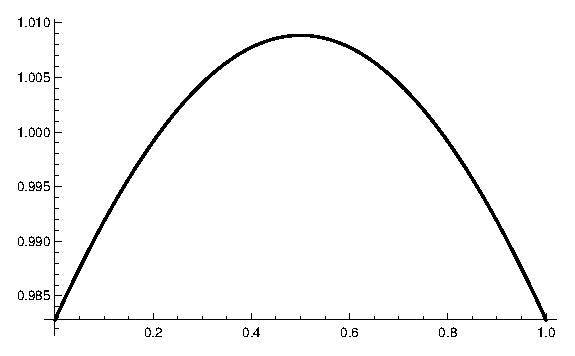
\includegraphics{chapters/appendices/KP_Mathematica/Kronig_Penney_model_transfer_matrix_gr8.eps}

\begin{doublespace}
\noindent\(\pmb{\text{pu2}=\text{Plot}[\text{Re}[\text{u2}[x,0.9,0.2]],\{x,0,1\},\text{PlotStyle}\to \{\text{Red},\text{Dashed}\}]}\)
\end{doublespace}

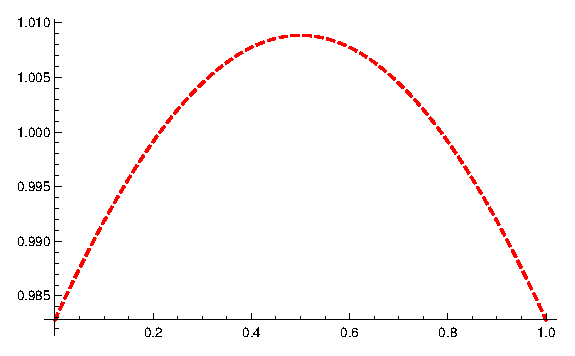
\includegraphics{chapters/appendices/KP_Mathematica/Kronig_Penney_model_transfer_matrix_gr9.eps}

\begin{doublespace}
\noindent\(\pmb{\text{Show}[\text{pu1},\text{pu2}]}\)
\end{doublespace}

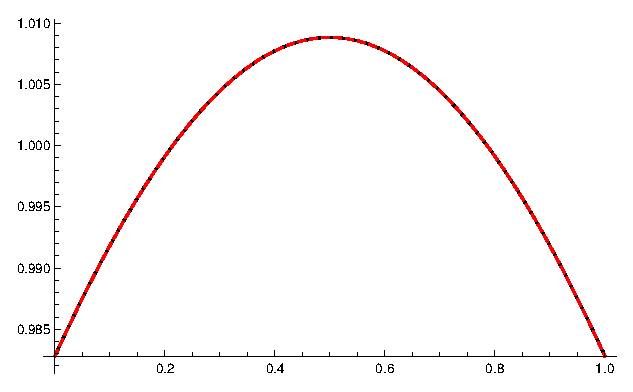
\includegraphics{chapters/appendices/KP_Mathematica/Kronig_Penney_model_transfer_matrix_gr10.eps}

\begin{doublespace}
\noindent\(\pmb{\text{(*} \text{plot} \text{imaginary} \text{part} \text{of} u(x) \text{*)}}\)
\end{doublespace}

\begin{doublespace}
\noindent\(\pmb{\text{pu3}=\text{Plot}[\text{Im}[\text{u1}[x,0.9,0.2]],\{x,0,1\},\text{PlotStyle}\to \text{Black}]}\)
\end{doublespace}

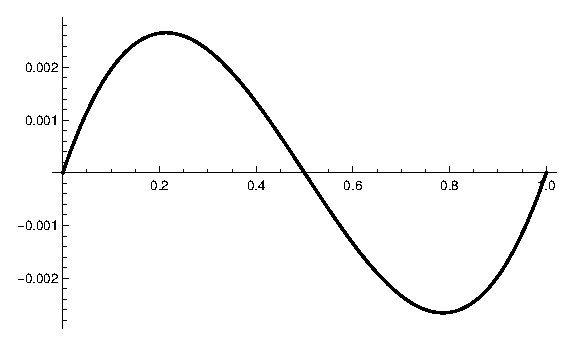
\includegraphics{chapters/appendices/KP_Mathematica/Kronig_Penney_model_transfer_matrix_gr11.eps}

\begin{doublespace}
\noindent\(\pmb{\text{pu4}=\text{Plot}[\text{Im}[\text{u2}[x,0.9,0.2]],\{x,0,1\},\text{PlotStyle}\to \{\text{Red},\text{Dashed}\}]}\)
\end{doublespace}

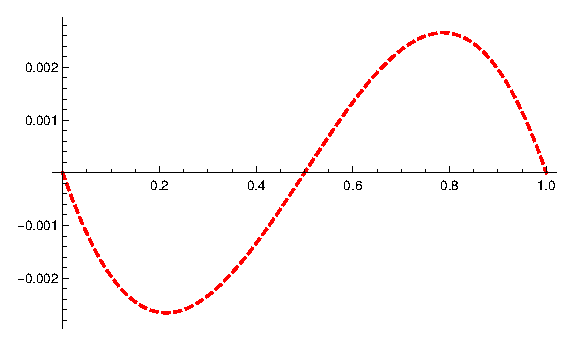
\includegraphics{chapters/appendices/KP_Mathematica/Kronig_Penney_model_transfer_matrix_gr12.eps}

\begin{doublespace}
\noindent\(\pmb{\text{Show}[\text{pu3},\text{pu4}]}\)
\end{doublespace}

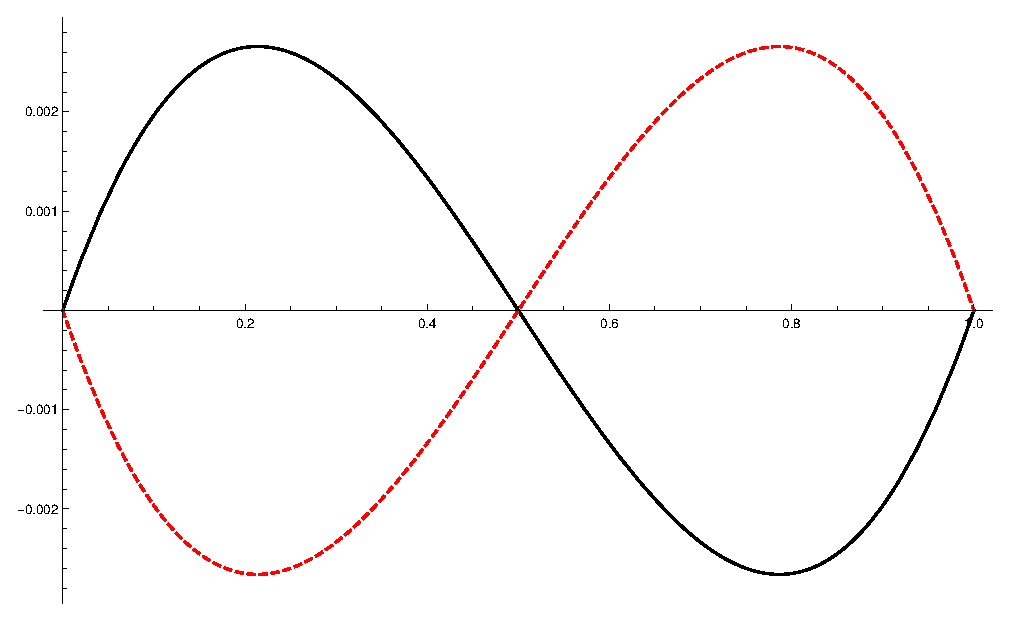
\includegraphics{chapters/appendices/KP_Mathematica/Kronig_Penney_model_transfer_matrix_gr13.eps}

\begin{doublespace}
\noindent\(\pmb{\text{}}\)
\end{doublespace}

\begin{doublespace}
\noindent\(\pmb{\text{(*} \text{Illustration}: \text{plot} u(x) \text{for} \text{epsilon} = 1 \text{and} q=2 \text{*)}}\)
\end{doublespace}

\begin{doublespace}
\noindent\(\pmb{\text{Abs}[\text{qq}[2,1]]\text{  }\text{//}N\text{   }\text{(*} \text{needs} \text{to} \text{be} <1 \text{*)}}\)
\end{doublespace}

\begin{doublespace}
\noindent\(0.188822\)
\end{doublespace}

\begin{doublespace}
\noindent\(\pmb{\text{u1}[0.4,2,1]}\)
\end{doublespace}

\begin{doublespace}
\noindent\(1.05025\, +0.0207882 i\)
\end{doublespace}

\begin{doublespace}
\noindent\(\pmb{\text{u2}[0.4,2,1]}\)
\end{doublespace}

\begin{doublespace}
\noindent\(1.05025\, -0.0207882 i\)
\end{doublespace}

\begin{doublespace}
\noindent\(\pmb{\text{(*} \text{plot} \text{real} \text{part} \text{of} u(x) \text{*)}}\)
\end{doublespace}

\begin{doublespace}
\noindent\(\pmb{\text{pu5}=\text{Plot}[\text{Re}[\text{u1}[x,2,1]],\{x,0,1\},\text{PlotStyle}\to \text{Black}]}\)
\end{doublespace}

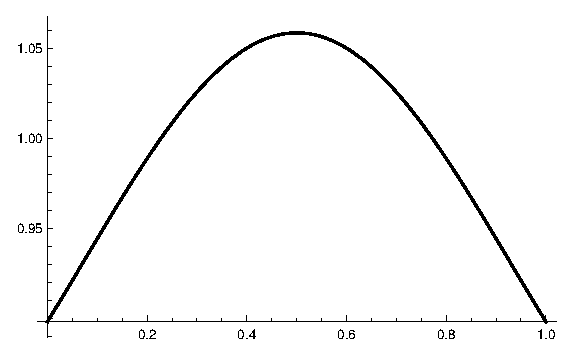
\includegraphics{chapters/appendices/KP_Mathematica/Kronig_Penney_model_transfer_matrix_gr14.eps}

\begin{doublespace}
\noindent\(\pmb{\text{pu6}=\text{Plot}[\text{Re}[\text{u2}[x,2,1]],\{x,0,1\},\text{PlotStyle}\to \{\text{Red},\text{Dashed}\}]}\)
\end{doublespace}

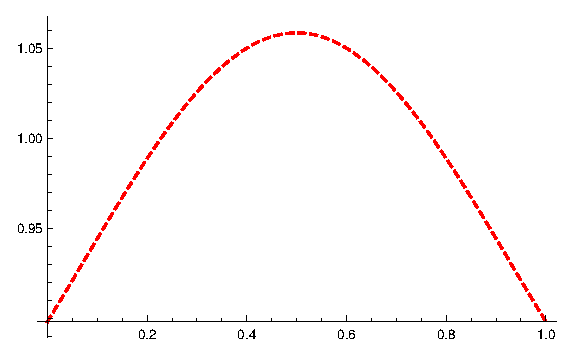
\includegraphics{chapters/appendices/KP_Mathematica/Kronig_Penney_model_transfer_matrix_gr15.eps}

\begin{doublespace}
\noindent\(\pmb{\text{Show}[\text{pu5},\text{pu6}]}\)
\end{doublespace}

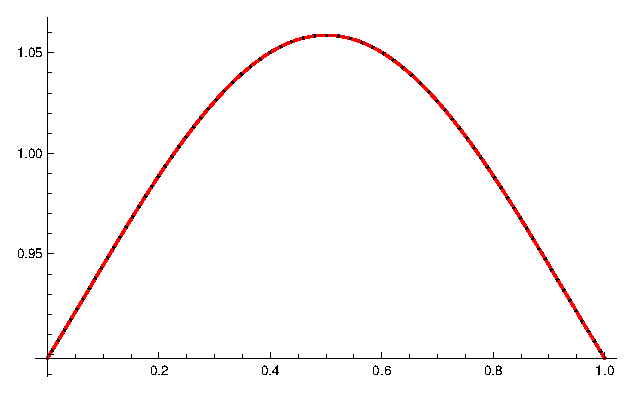
\includegraphics{chapters/appendices/KP_Mathematica/Kronig_Penney_model_transfer_matrix_gr16.eps}

\begin{doublespace}
\noindent\(\pmb{\text{(*} \text{plot} \text{imaginary} \text{part} \text{of} u(x) \text{*)}}\)
\end{doublespace}

\begin{doublespace}
\noindent\(\pmb{\text{pu7}=\text{Plot}[\text{Im}[\text{u1}[x,2,1]],\{x,0,1\},\text{PlotStyle}\to \text{Black}]}\)
\end{doublespace}

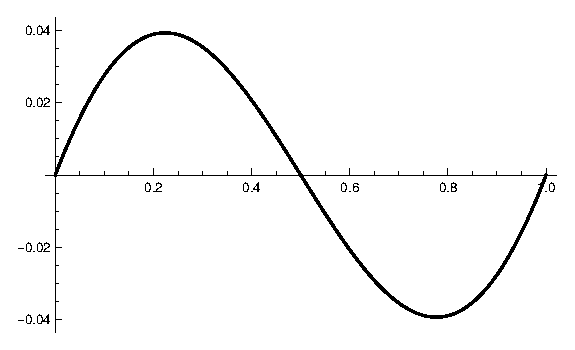
\includegraphics{chapters/appendices/KP_Mathematica/Kronig_Penney_model_transfer_matrix_gr17.eps}

\begin{doublespace}
\noindent\(\pmb{\text{pu8}=\text{Plot}[\text{Im}[\text{u2}[x,2,1]],\{x,0,1\},\text{PlotStyle}\to \{\text{Red},\text{Dashed}\}]}\)
\end{doublespace}

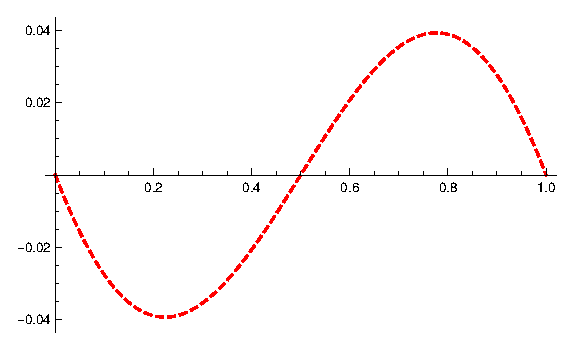
\includegraphics{chapters/appendices/KP_Mathematica/Kronig_Penney_model_transfer_matrix_gr18.eps}

\begin{doublespace}
\noindent\(\pmb{\text{Show}[\text{pu7},\text{pu8}]}\)
\end{doublespace}

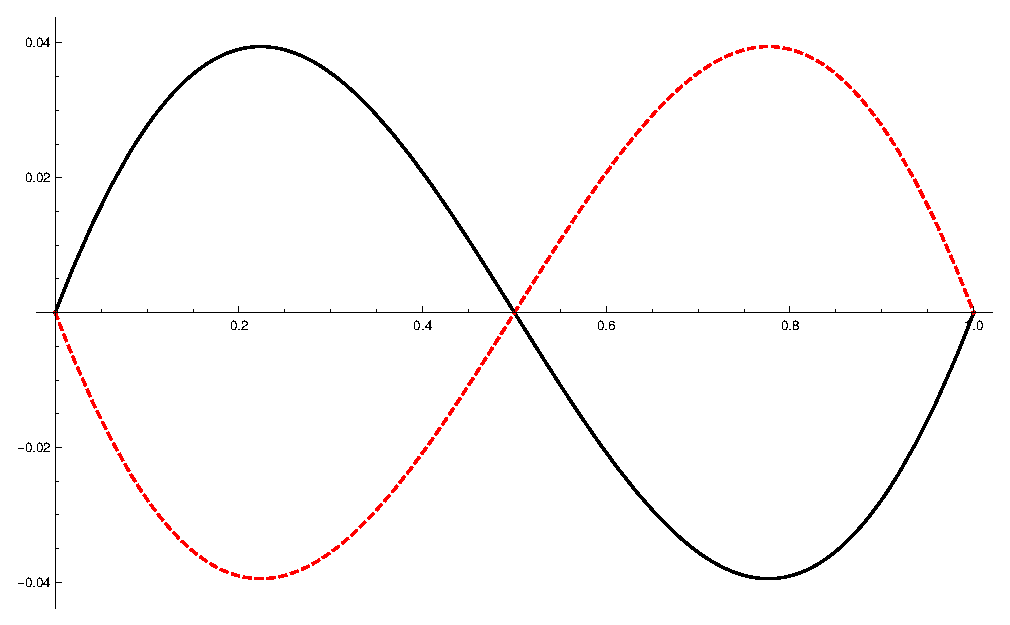
\includegraphics{chapters/appendices/KP_Mathematica/Kronig_Penney_model_transfer_matrix_gr19.eps}

\begin{doublespace}
\noindent\(\pmb{\text{}}\)
\end{doublespace}

\begin{doublespace}
\noindent\(\pmb{\text{Abs}[\text{qq}[1.1,1.348]]\text{    }\text{(*} \text{epsilon}=1.348 \text{is} \text{critical} \text{value} \text{for} q=1.1
\text{*)}}\)
\end{doublespace}

\begin{doublespace}
\noindent\(0.999663\)
\end{doublespace}

\begin{doublespace}
\noindent\(\pmb{\text{Plot}[\{\text{Re}[\text{u1}[0.4,1.1,\text{eps}]],\text{Re}[\text{u2}[0.4,1.1,\text{eps}]]\},\{\text{eps},0,2\},\text{PlotStyle}\to
\text{Black}]}\)
\end{doublespace}

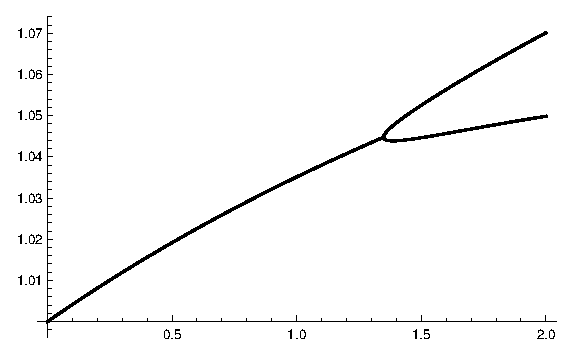
\includegraphics{chapters/appendices/KP_Mathematica/Kronig_Penney_model_transfer_matrix_gr20.eps}

\begin{doublespace}
\noindent\(\pmb{\text{Plot}[\{\text{Im}[\text{u1}[0.4,1.1,\text{eps}]],\text{Im}[\text{u2}[0.4,1.1,\text{eps}]]\},\{\text{eps},0,2\},\text{PlotStyle}\to
\text{Black}]}\)
\end{doublespace}

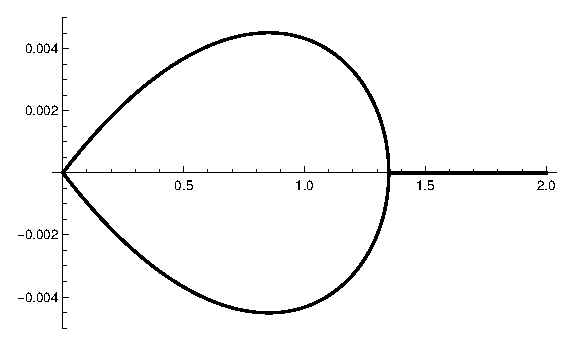
\includegraphics{chapters/appendices/KP_Mathematica/Kronig_Penney_model_transfer_matrix_gr21.eps}

\begin{doublespace}
\noindent\(\pmb{\text{}}\)
\end{doublespace}

\begin{doublespace}
\noindent\(\pmb{\text{(*} \text{Show}: \text{u2}'[0] = \text{Conjugate}[\text{u1}'[0]] \text{if} \text{Abs}[\text{qq}]<1 \text{*)}}\)
\end{doublespace}

\begin{doublespace}
\noindent\(\pmb{\text{Abs}[\text{qq}[0.9,0.2]]\text{    }\text{(*} \text{needs} \text{to} \text{be} <1 \text{*)}}\)
\end{doublespace}

\begin{doublespace}
\noindent\(0.708646\)
\end{doublespace}

\begin{doublespace}
\noindent\(\pmb{\text{u1prime}[0,0.9,0.2]}\)
\end{doublespace}

\begin{doublespace}
\noindent\(0.0982811\, +0.0269644 i\)
\end{doublespace}

\begin{doublespace}
\noindent\(\pmb{\text{u2prime}[0,0.9,0.2]}\)
\end{doublespace}

\begin{doublespace}
\noindent\(0.0982811\, -0.0269644 i\)
\end{doublespace}

\begin{doublespace}
\noindent\(\pmb{\text{Abs}[\text{qq}[2,3]] \text{//}N\text{   }\text{(*} \text{needs} \text{to} \text{be} <1 \text{*)}}\)
\end{doublespace}

\begin{doublespace}
\noindent\(0.265826\)
\end{doublespace}

\begin{doublespace}
\noindent\(\pmb{\text{u1prime}[0,2,3]}\)
\end{doublespace}

\begin{doublespace}
\noindent\(1.14432\, +0.624518 i\)
\end{doublespace}

\begin{doublespace}
\noindent\(\pmb{\text{u2prime}[0,2,3]}\)
\end{doublespace}

\begin{doublespace}
\noindent\(1.14432\, -0.624518 i\)
\end{doublespace}

\begin{doublespace}
\noindent\(\pmb{\text{(*} \text{END} \text{properties} \text{of} \text{u1}, \text{u2} \text{and} \text{derivatives} \text{*)}}\)
\end{doublespace}

\begin{doublespace}
\noindent\(\pmb{\text{}}\\
\pmb{}\)
\end{doublespace}

\begin{doublespace}
\noindent\(\pmb{\text{(*} \text{Plot} \text{real} \text{and} \text{imaginary} \text{parts} \text{of} \text{Bloch} \text{functions} \text{Phi$\_$raw}(x)
\text{*)}}\)
\end{doublespace}

\begin{doublespace}
\noindent\(\pmb{\text{(*} \text{Show} \text{Phi$\_$}2\text{$\_$raw} = \text{complex} \text{conjugate} \text{Phi$\_$}1\text{$\_$raw} \text{*)}}\)
\end{doublespace}

\begin{doublespace}
\noindent\(\pmb{\text{Abs}[\text{qq}[1,1]]\text{  }\text{//}N\text{  }\text{(*} \text{needs} \text{to} \text{be} <1 \text{*)}}\)
\end{doublespace}

\begin{doublespace}
\noindent\(0.961038\)
\end{doublespace}

\begin{doublespace}
\noindent\(\pmb{\text{p1}=\text{Plot}[\text{Re}[\text{phi1raw}[x,\text{Ceiling}[x],1,1]],\{x,0,20\},\text{PlotStyle}\to \text{Black}]}\)
\end{doublespace}

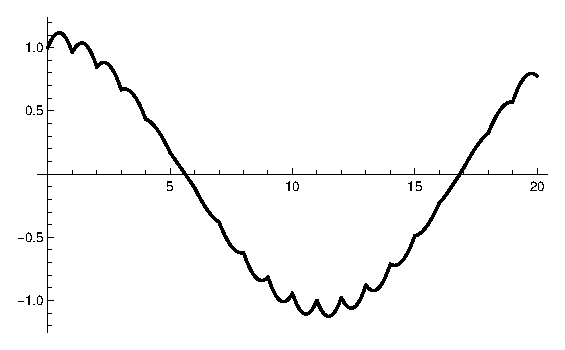
\includegraphics{chapters/appendices/KP_Mathematica/Kronig_Penney_model_transfer_matrix_gr22.eps}

\begin{doublespace}
\noindent\(\pmb{\text{p2}=\text{Plot}[\text{Re}[\text{phi2raw}[x,\text{Ceiling}[x],1,1]],\{x,0,20\},\text{PlotStyle}\to \{\text{Red},\text{Dashed}\}]\text{
 }\text{(*} \text{same} \text{as} \text{Re}(\text{phi1raw}) \text{*)}}\)
\end{doublespace}

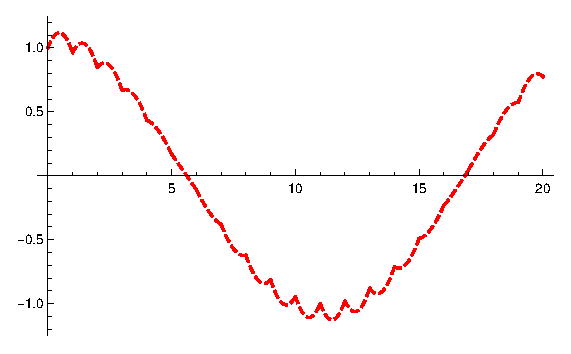
\includegraphics{chapters/appendices/KP_Mathematica/Kronig_Penney_model_transfer_matrix_gr23.eps}

\begin{doublespace}
\noindent\(\pmb{\text{Show}[\text{p1},\text{p2}]}\)
\end{doublespace}

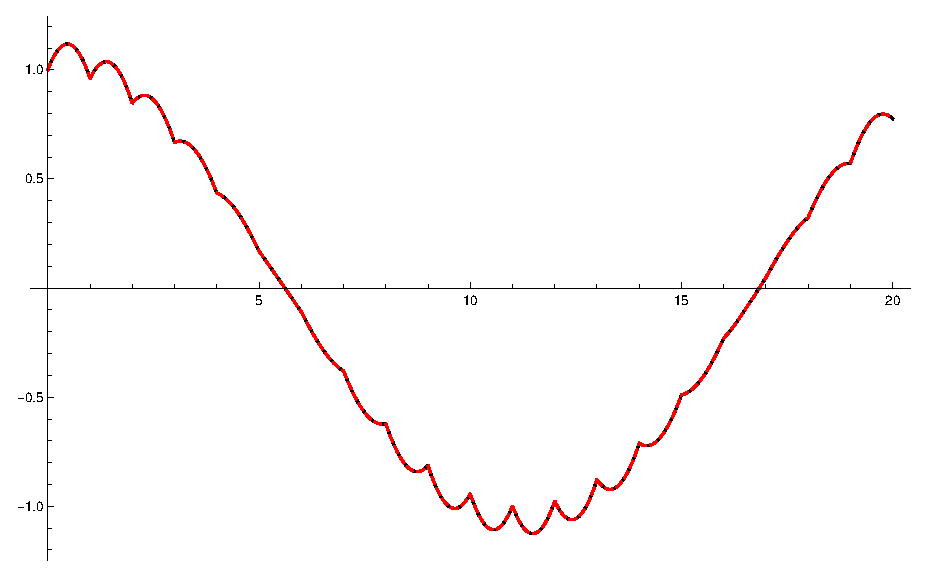
\includegraphics{chapters/appendices/KP_Mathematica/Kronig_Penney_model_transfer_matrix_gr24.eps}

\begin{doublespace}
\noindent\(\pmb{\text{p3}=\text{Plot}[\text{Im}[\text{phi1raw}[x,\text{Ceiling}[x],1,1]],\{x,0,20\},\text{PlotStyle}\to \text{Black}]}\)
\end{doublespace}

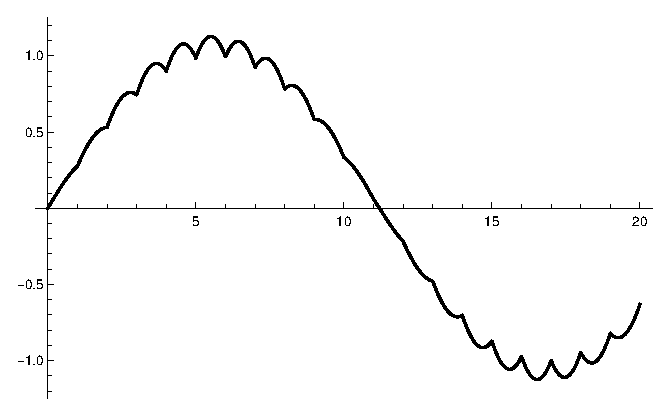
\includegraphics{chapters/appendices/KP_Mathematica/Kronig_Penney_model_transfer_matrix_gr25.eps}

\begin{doublespace}
\noindent\(\pmb{\text{p4}=\text{Plot}[\text{Im}[\text{phi2raw}[x,\text{Ceiling}[x],1,1]],\{x,0,20\},\text{PlotStyle}\to \{\text{Red},\text{Dashed}\}]\text{
 }\text{(*} -\text{Im}(\text{phi1raw}) \text{*)}}\)
\end{doublespace}

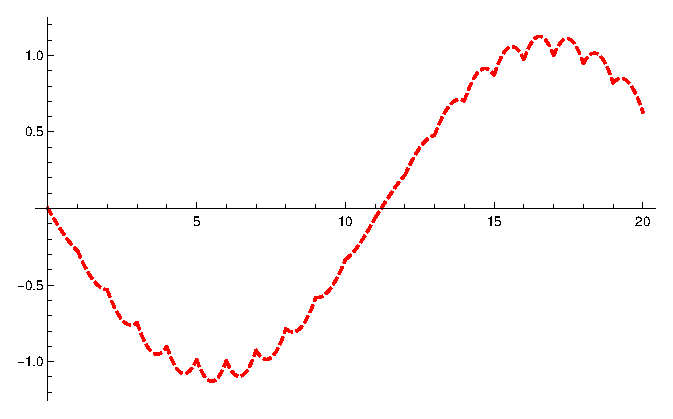
\includegraphics{chapters/appendices/KP_Mathematica/Kronig_Penney_model_transfer_matrix_gr26.eps}

\begin{doublespace}
\noindent\(\pmb{\text{Show}[\text{p3},\text{p4}]}\)
\end{doublespace}

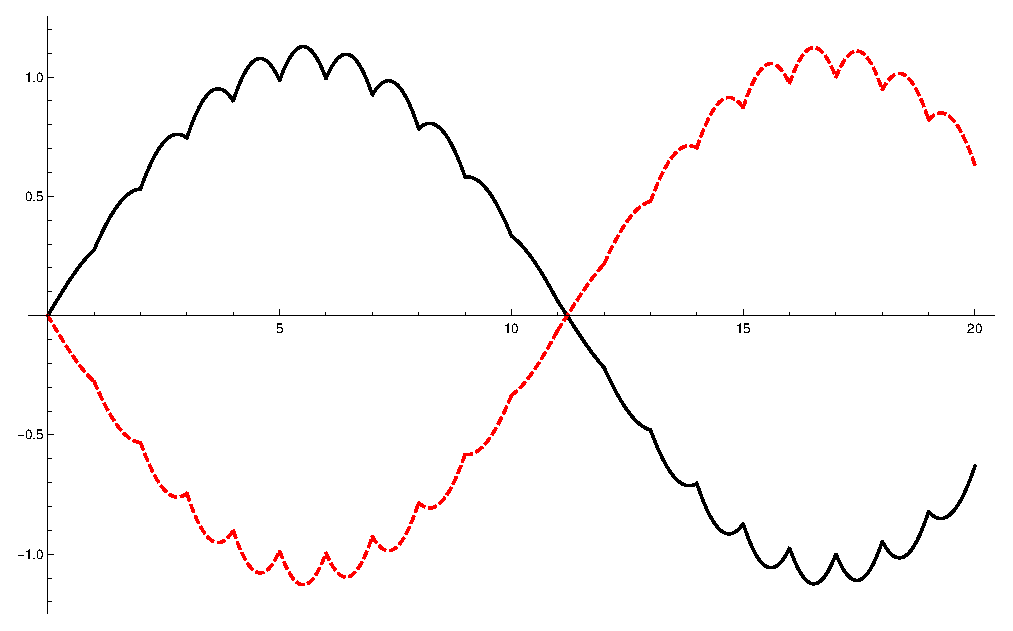
\includegraphics{chapters/appendices/KP_Mathematica/Kronig_Penney_model_transfer_matrix_gr27.eps}

\begin{doublespace}
\noindent\(\pmb{\text{}}\\
\pmb{}\\
\pmb{}\\
\pmb{}\)
\end{doublespace}

\begin{doublespace}
\noindent\(\pmb{\text{(*} \text{Show} \text{that} \text{phi1raw}(x=n,n,q,\text{epsilon}) = \text{Exp}(i k n) \text{*)}}\)
\end{doublespace}

\begin{doublespace}
\noindent\(\pmb{\text{phi1raw}[7,7,0.9,0.2] \text{//}N}\)
\end{doublespace}

\begin{doublespace}
\noindent\(0.696237\, -0.717812 i\)
\end{doublespace}

\begin{doublespace}
\noindent\(\pmb{\text{Exp}[I \text{kk}[0.9,0.2] 7]\text{  }\text{//}N}\)
\end{doublespace}

\begin{doublespace}
\noindent\(0.696237\, -0.717812 i\)
\end{doublespace}

\begin{doublespace}
\noindent\(\pmb{\text{phi1raw}[8,8,2,3] \text{//}N}\)
\end{doublespace}

\begin{doublespace}
\noindent\(-0.549437-0.835535 i\)
\end{doublespace}

\begin{doublespace}
\noindent\(\pmb{\text{Exp}[I \text{kk}[2,3] 8]\text{  }\text{//}N}\)
\end{doublespace}

\begin{doublespace}
\noindent\(-0.549437-0.835535 i\)
\end{doublespace}

\begin{doublespace}
\noindent\(\pmb{\text{}}\)
\end{doublespace}

\begin{doublespace}
\noindent\(\pmb{\text{(*} \text{Show} \text{that} \text{phi2raw}(x=n,n,q,\text{epsilon}) = \text{Exp}(-i k n) \text{*)}}\)
\end{doublespace}

\begin{doublespace}
\noindent\(\pmb{\text{phi2raw}[7,7,0.9,0.2] \text{//}N}\)
\end{doublespace}

\begin{doublespace}
\noindent\(0.696237\, +0.717812 i\)
\end{doublespace}

\begin{doublespace}
\noindent\(\pmb{\text{Exp}[-I \text{kk}[0.9,0.2] 7]\text{  }\text{//}N}\)
\end{doublespace}

\begin{doublespace}
\noindent\(0.696237\, +0.717812 i\)
\end{doublespace}

\begin{doublespace}
\noindent\(\pmb{\text{phi2raw}[8,8,2,3] \text{//}N}\)
\end{doublespace}

\begin{doublespace}
\noindent\(-0.549437+0.835535 i\)
\end{doublespace}

\begin{doublespace}
\noindent\(\pmb{\text{Exp}[-I \text{kk}[2,3] 8]\text{  }\text{//}N}\)
\end{doublespace}

\begin{doublespace}
\noindent\(-0.549437+0.835535 i\)
\end{doublespace}

\begin{doublespace}
\noindent\(\pmb{\text{}}\)
\end{doublespace}

\begin{doublespace}
\noindent\(\pmb{\text{(*} \text{Illustration}: \text{Geshkenbein} \text{Fig}. 1 \text{*)}}\)
\end{doublespace}

\begin{doublespace}
\noindent\(\pmb{f[\text{k$\_$}]\text{:=}\text{Cos}[k]+\text{epsilon}/(2k) \text{Sin}[k]}\)
\end{doublespace}

\begin{doublespace}
\noindent\(\pmb{f[k]}\)
\end{doublespace}

\begin{doublespace}
\noindent\(\text{Cos}[k]+\frac{5 \text{Sin}[k]}{k}\)
\end{doublespace}

\begin{doublespace}
\noindent\(\pmb{\text{plus}[\text{k$\_$}]\text{:=}1}\)
\end{doublespace}

\begin{doublespace}
\noindent\(\pmb{\text{minus}[\text{k$\_$}]\text{:=}-1}\)
\end{doublespace}

\begin{doublespace}
\noindent\(\pmb{\text{epsilon}\text{:=}10\text{   }\text{(*} \text{value} \text{for} v=\text{epsilon} \text{used} \text{in} \text{Geshkenbein} \text{Fig}.
1 \text{*)} }\)
\end{doublespace}

\begin{doublespace}
\noindent\(\pmb{\text{pp1}=\text{Plot}[\{f[k],\text{plus}[k],\text{minus}[k]\},\{k,0,19\},\text{PlotRange}\to \{\{0,19\},\{-2,2\}\},\text{PlotStyle}\to
\text{RGBColor}[1,0,0]]}\)
\end{doublespace}

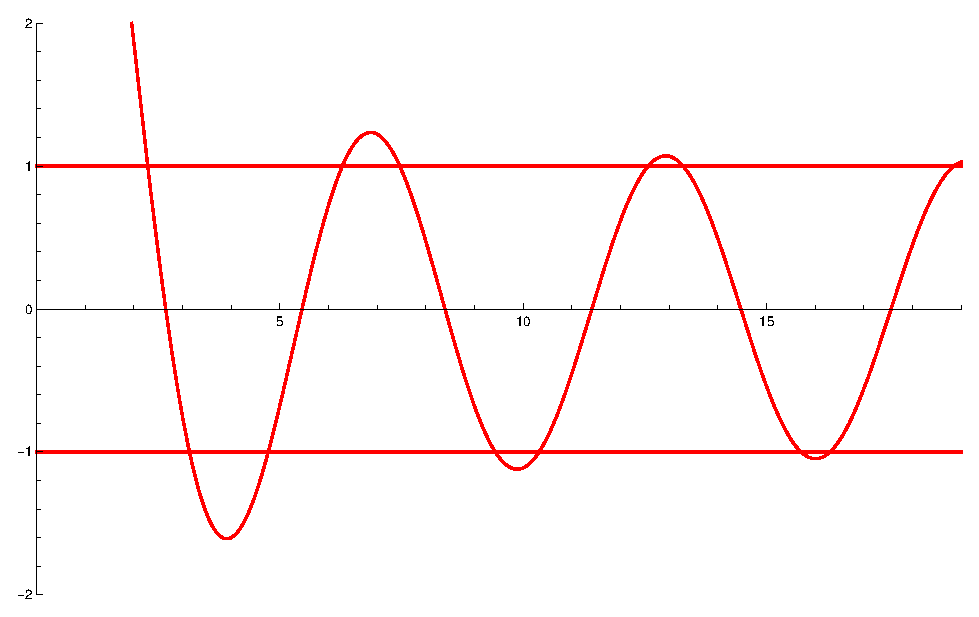
\includegraphics{chapters/appendices/KP_Mathematica/Kronig_Penney_model_transfer_matrix_gr28.eps}
